\documentclass[pdftex,12pt,a4paper]{article}
\usepackage[pdftex]{graphicx}
\usepackage{xcolor}
\usepackage{marginnote}
\usepackage{enumitem}
\usepackage{multirow}
\usepackage{subcaption}
\usepackage{titlesec}
\usepackage[bottom=1.5cm, outer=5cm, inner=2cm, heightrounded,
marginparwidth=4cm, marginparsep=0.5cm]{geometry}
\titleformat{\section}{\bfseries}{\Large Question \thesection: }{0em}{}

\begin{document}
    % Custom title page
    \begin{titlepage}
        \begin{center}
            
\includegraphics[width=5cm]{figures/kulogo}\\[1cm]
            {\large \bfseries
                Spring 2014\\
                Computer Networks\\
                CMPE323\\[1cm]
            }
            {\large \bfseries
                \noindent Quiz 1 (2$^{nd}$ Group)\\[1cm]
            }
        \end{center}

        \begin{center}
            \begin{tabular}{|c|p{1cm}l|}\hline
                \textbf{Questions} & \multicolumn{2}{|c|}{\textbf{Points}} \\\hline
                Q1                &    &    /25\%   \\
                Q2                &    &    /25\%   \\
                Q3                &    &    /25\%   \\
                Q4                &    &    /25\%   \\\hline
                Total             &    &    /100\%  \\\hline
            \end{tabular}
        \end{center}

        \vfill
        \begin{tabular}{lp{5cm}ll}
            \textbf{Student name:} & & \textbf{Student ID:} & \\
        \end{tabular}


    \end{titlepage}
    \newpage

    % quiz content
    \section{}
        Suppose that we have two PCs (PC1 and PC2) that are directly connected to each
        other via their Ethernet network adapter, then which one of the
        following pin-arrangements will allow their connectivity given that
        Auto-MDIX is disabled:

        \begin{figure}[tbh]
            \centering
            \begin{subfigure}{.5\textwidth}
              \centering
              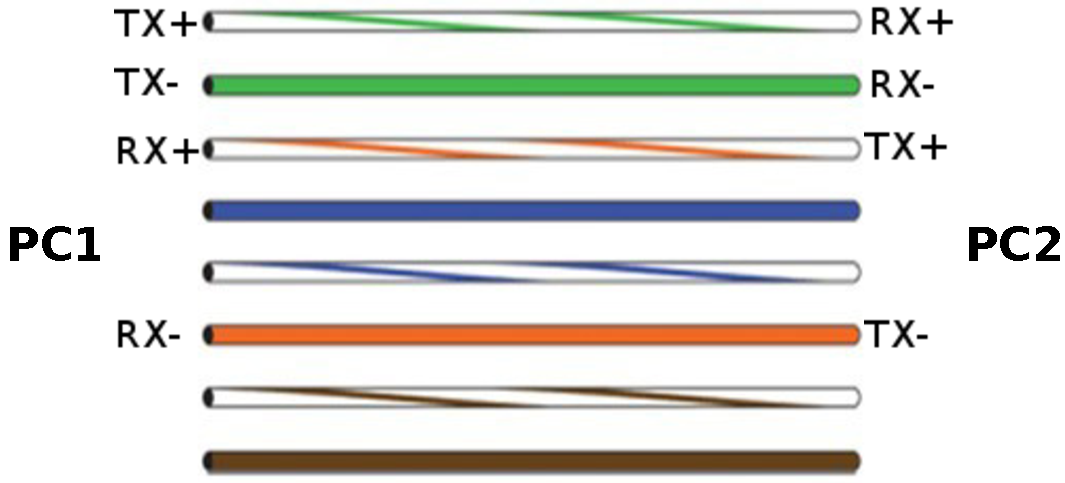
\includegraphics[width=.95\textwidth]{figures/fig1a}
              \caption{\ }
              \label{fig:sub1}
            \end{subfigure}%
            \begin{subfigure}{.5\textwidth}
              \centering
              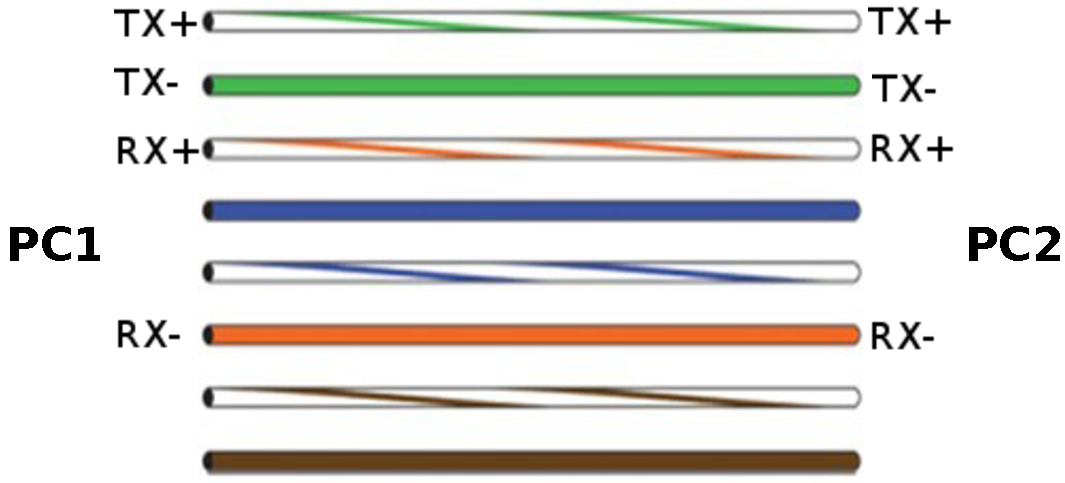
\includegraphics[width=.95\textwidth]{figures/fig1b}
              \caption{\ }
              \label{fig:sub2}
            \end{subfigure}
              \vspace{30pt}

            \begin{subfigure}{.5\textwidth}
              \centering
              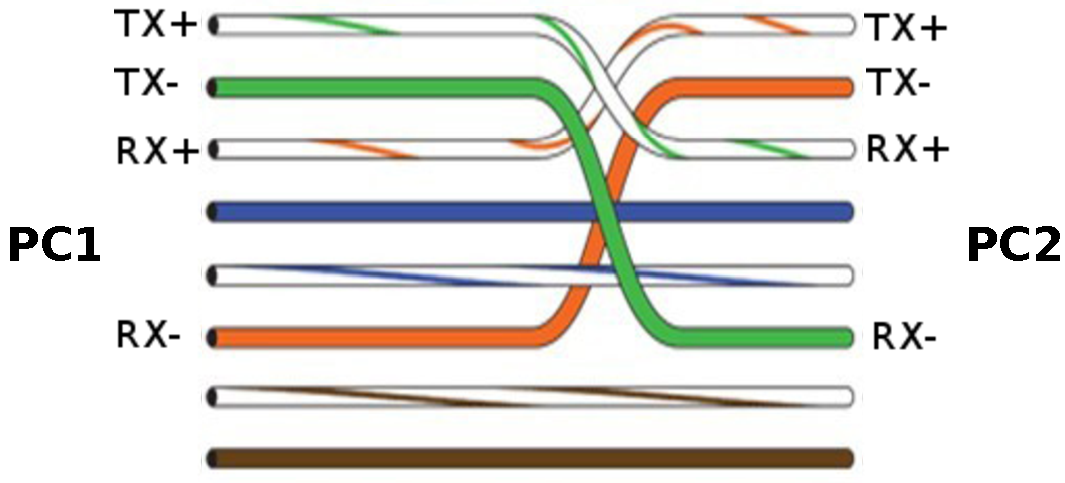
\includegraphics[width=.95\textwidth]{figures/fig1c}
              \caption{\ }
              \label{fig:sub3}
            \end{subfigure}%
            \begin{subfigure}{.5\textwidth}
              \centering
              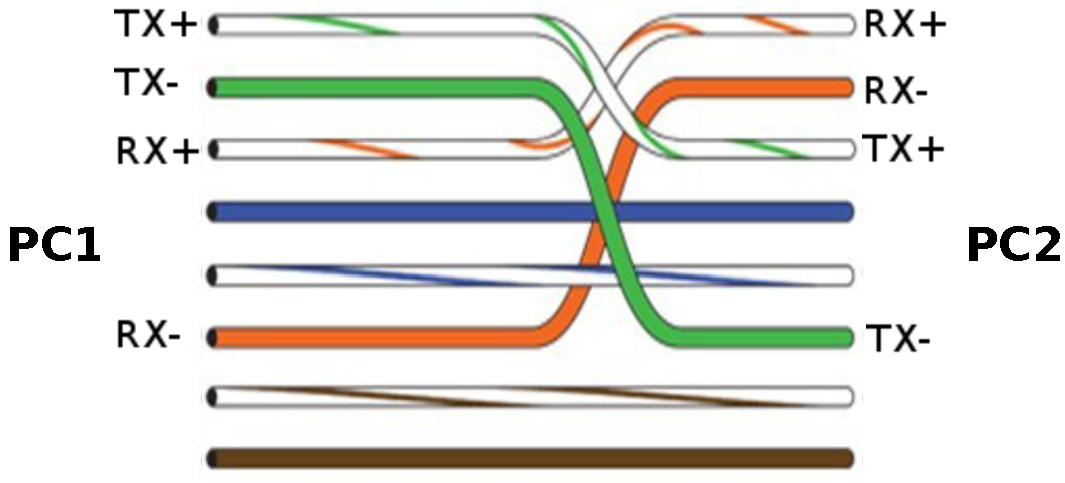
\includegraphics[width=.95\textwidth]{figures/fig1d}
              \caption{\ }
              \label{fig:sub4}
            \end{subfigure}
        \end{figure}

        \newpage

    \section{}
        Considering the single broadcast domain network that is presented in
        Figure \ref{fig:bd}, if the Ethernet switch received from its
        \texttt{fa0/2}
        interface a MAC frame with
        a destination MAC address of \texttt{00:00:00:00:00:02}, which port(s) will
        the switch forward the frame to?

        \begin{figure}[tbh]
            \centering
            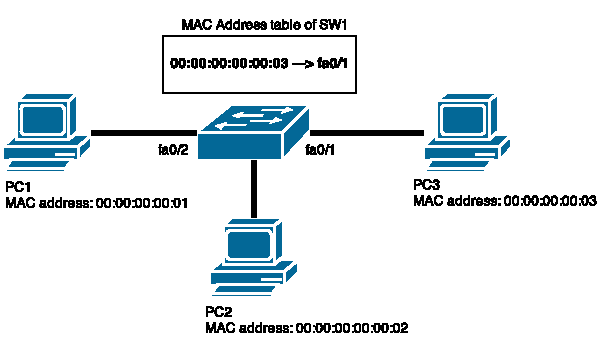
\includegraphics[width=0.85\textwidth]{figures/diag1.pdf}
            \caption{A single Ethernet broadcast domain connecting PC1, PC2 and PC3.}
            \label{fig:bd}
        \end{figure}

        \newpage

    \section{}
        Considering the broadcast domains as presented in Figure
        \ref{fig:vlan}, if PC1 sends a broadcast MAC frame with the destination
        MAC address of \texttt{FF:FF:FF:FF:FF:FF}, which PC(s) will receive the message?
        \begin{figure}[tbh]
            \centering
            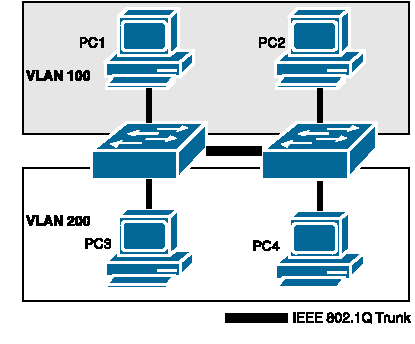
\includegraphics[width=0.65\textwidth]{figures/diag2.pdf}
            \caption{Two separate Ethernet broadcast domains connecting PC1,
            PC2, PC3 and PC4.}
            \label{fig:vlan}
        \end{figure}

        \newpage

    \section{}
        Assuming that all devices (PCs and routers) in IP network as presented
        in Figure \ref{fig:ip} are configured correctly with the exception that R1
        is unable to reach the network \texttt{10.0.3.0/24}. What entry should
        be added in R1's routing table in order to solve this reachability
        issue?
        \begin{itemize}
            \item Network IP address:
            \item Network subnet mask\footnote{You can express it as bits (e.g.
                /24) or 4-octet addresses (e.g. 255.255.255.0).}:
            \item Gateway\footnote{Also known as next-hop node.} IP address:
        \end{itemize}

        \begin{figure}[tbh]
            \centering
            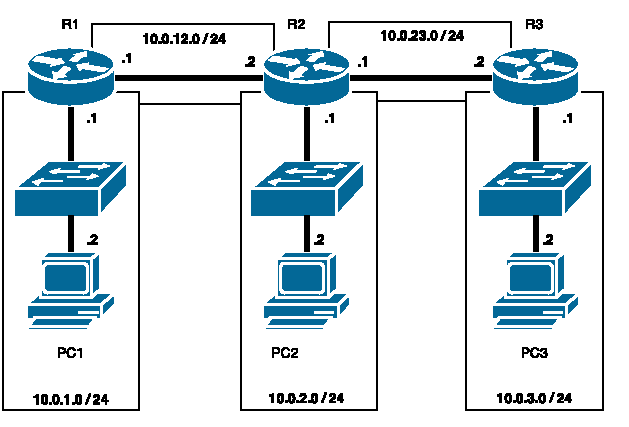
\includegraphics[width=0.95\textwidth]{figures/diag3.pdf}
            \caption{Various Ethernet broadcast domains being inter-connected
            via 3 IP routers.}
            \label{fig:ip}
        \end{figure}

        \newpage


\end{document}
